\chapter{Skill Design} %\inote{ (was: Implementation) Dienstabfrage}}
\label{mainone}
%DELETEME: In this chapter you start addressing your actual problem. Therefore, it makes often sense to make a detailed problem analysis first (if not done in introduction). You should be sure about what to do and how. As writtin in the background part, it might also make sense to include complex background information or papers you are basing on in this analysis. If you are solving a software problem, you should follow the state of the art of software development which basically includes: problem analysis, design, implementation, testing, and deployment. Maintenance is often also described but I believe this will not be required for most theses. Code should be placed in the appendix unless it is solving an essential aspect of your work.




This chapter lays out the first details of our Skill implementation. We discuss the choices we need to take and why we take them in the first section, going over the framework requirements in which we do this implementation, to finally introduce the interaction model, also known for being the skill configuration, based on which we fulfill the intents in the Skill's back-end implementation (Chapter \ref{maintwo}). We also provide guidance on best practices during the whole process in Section \ref{designGuide}.

Before proceeding, we state that Alexa gives the limitation of recording audio for transcription at a bit rate of 8kHz using the file formats LPCM and Opus for input and MPEG, OGG and PCM for output. Using the Skill is only possible through an internet connection. There are options to keep the context (session) alive for only 8 seconds, extendible by another 8 second for re-prompts to give the user enough time to think and answer. and Finally, knowing that Alexa uses term weighting to understand the user, we are able to find out what utterances were missed, e.g. through the options described previously in Chapter \ref{amznecosys}. 


%
%Abtastrate für Telefon-Audio (8 kHz)
%Amazon Lex unterstützt die folgenden Formate für den Audioeingang: LPCM und Opus. 

%
%Verwendung nur über das Internet möglich
%
%behalten den Kontext
%It tells you what utterances were missed





%\todo{
%	intro on structure of chapter\\
%- to then elaborate on implementation requirements in section \ref{frameworks_structs}. 
%- functional requirements (although this is not OCL now, but requiring an SSL cert.) / non-functional (bot muss höflich sein)
%}





%
%\todo{
%	%this is mostly repeating intro saying that you found a solution for the requirements
%	- ..it would speak as an advantage for bots if they can determine these things automatically..\\
%	%	mentioned earlier - imagination about ablitiy to react to everything\\
%	- currently most tasks revolve around performing tasks like setting an alarm, 
%	%	to perform task like - mention top 10 and a few more stats / tech review
%	- answer suggestions functionality in chatbot equivalent
%	- next step is to get around the user's frustration by making the bot at least more human.	
%	
%	- Alexa Skill will work in Germany in english and german -> add english after german
%}




%
%
%\todo{MAGENTA\\
%	-AL: Ich w\"urde erst etwas die Algorithmen und Datenstrukturen (Textanalyse, JSON, ggf. Graphen beschreiben). \\
%	-AL: Anschlie{\ss}end die Frameworks vorstellen\\ 
%	-AL: Wichtig ist: Aus den Beschreibungen eine Schlussfolgerung ableiten, welche Art von L\"osung entwickelt werden soll.\\
%	for current bot: \\
%	- Lucene \textbf{as the golden standard}: spell check, unscharfe suche, Tika / detect language / ... \\
%	- Solr
%	- explain what's an intent, whats a slot
%	\url{https://service.berlin.de/virtueller-assistent/virtueller-assistent-606279.php}
%	\url{https://www.itdz-berlin.de/}
%}
%






\section{Design Choices}



Skill design is crucial for the later development stages, as it gives us an overview of what we want to achive and how we want to achive it. It is therefore essential to start with before implementing the fulfilment part. A few questions necessary for the design process are:
\begin{itemize}
\item \textbf{What should the Skill do?\\}
In our case: Look up information about services and book appointments.
\item  \textbf{How should it do it?\\}
In our case: It should connect to the API, make GET requests to receive the most recent information and read out the relevant parts from the JSON nodes (as the response's structure was discussed earlier in Table \ref{dienstleistung:descr}), while maintaining a conversational flow that is not redundant or too complex to the user. In a next step, it should also be able to create appointments on Berlin.de's endpoint through POST requests connect to the user's calendar to save these.

\item \textbf{Through what conversational interaction does the user get to invoke that action?}\\
In our case: The user can ask Alexa directly to book an appointment or get to find out more about the service through a series of questions (Multi-turn conversation, see Section \ref{multiturn:def}).

\end{itemize}


Although this process sounds simple, putting oneself in the mindset of a developer and creating a scenario requires extensive preparation, as there are possibly endless options of how a user can describe what they want to do. As we opt for Alexa, we explore what options it offers to minimise the developer's work on predicting utterances and how paths are built to reach the intents. We also discover the role of synonyms in sentence wording. Further, in the process, we touch on the frameworks we can make use of in this step.


	
	\begin{wrapfigure}{r}{0.48\textwidth}
		\caption[Hook Model Steps]{The Hook Model: four key steps for creating products that users can crave. Based on \cite{eyal:hook}}
		\label{hookeyal}
		\includegraphics[width=7cm]{hook}
	\end{wrapfigure}

Beyond the academic research, with releasing the Skill as a target in mind, Eyal's hook model \cite{medium:skillmarketing} is of strategic value for reference throughout. In his book ``Hooked: How to Build Habit-Forming Products'', he describes hooks as “experiences designed to connect the user’s problem with the company’s product with enough frequency to form a habit'' \cite{eyal:hook}.
%
%\end{itemize}  in the \href{https://medium.com/the-mission/nobody-cares-about-your-amazon-alexa-skill-ac14bd080327}{nobody cares abt ur skill}
%
%
In our Skill context, we observe from our own questionnaire as well as in another study findings by Experian Information Solutions, Inc. \cite{experian} that 
most tasks in Alexa currently revolve around performing simple actions like setting a timer or playing specific music.
Although it would speak as an advantage for a voice assistant if it can automatically determine more context, we use this as a guideline for keeping the actions short and simple.
%	mentioned earlier - imagination about ablitiy to react to everything\\
%- currently most tasks revolve around performing tasks like setting an alarm, 
%	to perform task like - mention top 10 and a few more stats / tech review
%- answer suggestions functionality in chatbot equivalent

\subsection*{Sentence length}
For this we use a maximum of two sentences per action and keep them not shorter than three words (e.g. ``I want \mintinline{java}{service_name}'') and not longer than 30 words, with an of 10 words that a user needs to make sure they get the appropriate answer.
As we know it is common to miss the correct intent, we implement an  \mintinline{java}{Unhandled} intent. This is not a must but it assures that we 
%The next step is to 
attempt to get around the user's frustration by making the bot at least more human in the answers it gives if no intent was found.	

\subsection*{Skill availability,  languages and dialects used}
Since we see the demand for both English and German prevalent in the survey, we start with a German model and implement in the equivalent english model services that are more related to residents of foreign countries, since the service catalogue is more relevant to this audience (e.g. residence permits, transfer or driving licence, registration).
%- Alexa Skill will work in Germany in english and german -> add english after german



We choose to offer our skill only in Germany because our Skill's functionality is specific only within this geographical region. For that we configure the Skill to handle English (US) and German (Germany).
At the time of development, Alexa was more able to understand an American dialect than a British one.
Consequently, we draft two interaction models, each with an intent handler, which we register based on the user's device's language. This is to avoid errors in case one intent is found in both language models with the same intent.
There are other solutions possible, but this choice remains as a more systematic one for error handling and coherent code placement.


%\todo{\textit{moved from availability section in choice of platform:}\\

%	say why we do it like this 3ashan each language group has a different interest although we can do a handler function for two languages but we prefer not to 3ashan ne3melha schöne und nicht systematische implementierung.
%}



\subsection*{Addressing the user}
Although this might conflict with the way Alexa addresses the users in German, we also use the formal `Sie' since this is the same language our API uses. This is a non-functional requirement we also infer form the D115 whitepaper\cite{d115}



\subsection*{Skill extent}
With modularity as an underlying concept, we keep the Skill's range to providing information and potentially booking appointments as the major hook element. Any information related to current events in the city should be within the perimeter of another Skill in order not to overload the interaction model, which could result in the Skill not understanding the user. Further, though this could be done by a parser, the API does not support more than providing information at the time of development.

This coincides with giving a hook for this skill and any other skill revolving around the user's entertainment.




\subsection*{Session duration}
\label{sessionduration}
With A-B tests we determine the optimal duration of a session (8 vs. 16 seconds) based on each question. and do not apply a general rule for it. The upside of keeping a session longer is that the conversation context will remain longer. On the downside, it might clog the user from using Alexa in a different context as well as giving the impression of `spying' on the user for an extended time if it is not necessary to keep the session alive. Adjusting whether the session should remain for an extended time happens through the JSON request property \mintinline{javascript}{{'ShouldEndSession' = 'false'}}


\subsection*{Alexa's reprompts and utterances}
We randomise what Alexa says in some situations, where the user would prefer not to hear the same answer every time they reach a certain conversational path. In other path junctions, we give out the same spoken text for the user to get a sense of familiarity on where they are in the conversation. This keeps a balance between clarity and spontaneity 


\subsection*{Help}
We offer various ways to provide the user with help. On one hand we implement an extensive \mintinline{java}{HelpIntent} that gives a help menu to the user, suggests Intents to speak through audio and on the device's display. We also provide contextual help within each intent. Helps usually require randomising sentences to users for them to know what they are capable of with the Skill.


%
%
%
%\todo{
%	then talk about how you researched on alexa's available skills and found out that the e-Government sector is underrepresented and hence you chose this as ur analyzed scenario.\\
%	%%% move to section \ref{choiceOfPlatform}
%	fluidly contiuning from intro and background:\\
%	- since among Apple and Google it hast the voice-first devices best equipped for its platform, a user base larger then its competition and provides the most mature API and SDKs.\\
%	
%	- We choose this skill scenario since it is underrepresented in that pie chart. ... 
%	- amazon as a platform is compared to apple and google readiest (check ref voicelabs)
%}
%
%
%\todo{
%	It's important to say that they do not transcribe, but do term weighting etc, a black box, and that we will not hear everything right, just as we as humans do not}
%
%


%option: make two versions of it - wa7ed only focused on the info, the other is a module on top of it for entertainment

%How to optimize, e.g. making a longer session
%- z.B. with this Microsoft way to make a bot session last for a long time and start a session w keda 3ashan ye3mel sense of the context around it (conversation before and after)
%- give a suggested answer



%developer’s role:
%clarity
%spontenaety
%competence

After all, the user should feel the competence of the Skill to be convinced of using it. % which means they would speak 
As such, we need to create an interaction model that takes care of wording order and a fulfilment that has competent error handling paths. 

\subsection*{What intents represent}
 As it is better to separate utterances by intents (Section \ref{designGuide}), we start with an utterance, see which intent it can relate to. 
 There are several ways to structure intents, depending on how we define them. After many trials on the categorisation of intents, we group intents based on what a user's question revolves about in each of the topics. Hence, the intents map to the sections of the Berlin City Portal service sections:
 \begin{itemize}
 	\itemsep0em
\item General Inquiry
\item Prerequisites
\item required documents
\item Costs
\item Processing Time
 \end{itemize}
 
 Other sections like `legal base' or `forms' are not of added value and will not be spoken out to the user.
 
 Additionally, since many public services are related to one another, we group similar ones by goal. For instance, `registration' and `de-registration' could have an analogous sound with 8Kbps, especially in German (`Anmelden' vs. Ambelden or Ummelden). Making a special intent for this service helps determine the right service through confirmation. Other services like Applying for a student loan (BAFöG) is available in the service catalogue under different services depending on the target group (student, school pupils, apprentice, loan for a study-abroad) and requires further questions as not every user is expected to recite the type of BAFöG they want in the first utterance.



\subsection*{Synonyms}
Usage of synonyms depends on where the synonym can be used. For instance when we expect the user to ask for `ID' instead of an `ID Card' (the full service name), In another example, where we expect the user to answer to the `kind of doctor', in German the words `Tierarzt' (Veterinarian ), `Hausarzt' (General Practitioner), `Augenarzt' (Optician) and `Zahnarzt' (Dentist) are all derived from the same job description `Arzt' (Doctor). In our implementation, where the user is not expected to ask a question related to a veterinarian, we omit the synonym `Tierarzt'.

This is one example that shows how each model should represent no more than one language locale, as synonyms and phrases differ between locales.


\subsection*{Slot Types}
Many of the slot types are not available on Amazon, which means we have to create them. We transpose some of the lists obtained from the Virtual Citizen Assistant and create our own based on other formats provided either through csv files (e.g. for PLZ values) or through the parsing the berling website directly and importing the list into a slot type with minimal string modifications to match our model requirements (e.g. with Citizenships). Problems with this approach are discussed in Section \ref{challenges:design}. \\





The complete model is provided with the Skill code as a JSON file named as the locale of the model (\mintinline{bash}{de_DE.json} and \mintinline{bash}{en_US.json}). attached to this research. In Figure \ref{interactionModel:bild}, a representation thereof via Alexa Skills Kit interface. Table \ref{interactionModel} highlights representative elements included in the model schema.

\begin{figure}[h!]
	\centering
	\caption[Interaction Model]{A representation of the designed interaction model}
	\label{interactionModel:bild}
		\includegraphics[width=\linewidth]{interactmo}
		
		  
\end{figure}

%
%\todo{dann UML Diag showing interaction}


\begin{table}[h!]
	\caption[Interaction Model Schema]{\href{https://developer.amazon.com/docs/smapi/interaction-model-schema.html}{Interaction Model Schema (Skill Management API)~\cite{alexaDesignGuide} }}\label{interactionModel}
	
	\begin{tabularx}{\textwidth}{l | l l l  }
		Field	&	Type	&	Description		&	Required \\ \hline \hline
		\lstinline|languageModel| &	object	& Conversational primitives for the skill	& Yes\\
		\quad\lstinline|invocationName| &	object	& Invocation name of the skill	& Yes\\
		\quad\lstinline|intents| &	array	& Intents and their slots	& Yes\\
		\quad\quad\lstinline|slots|  & array & List of slots within the intent	& No\\
		\quad\lstinline|types| &	array	& Custom slot types		& No\\
		\quad\quad\lstinline|samples|	& array	 & Sample utterances for the intent	& No\\
		
		\lstinline|dialog| & object & Interaction, slot filling, confirmations & No\\
		\quad \lstinline|confirmationRequired| & value & \shortstack[l]{flag to set if Alexa will confirm\\ with a statement once a slot is caught}& Yes \\
		\lstinline|elicitationRequired| & value & flag if required & Yes\\
		\lstinline|elicitation| & value & \shortstack[l]{pointer to elicitation value to register if  \\  more than one Intent found for slot}  & \\
%		\lstinline|type| (slot type) & & & \\
%		\lstinline|name| (slot name) & & & \\		
		\lstinline|prompts| & array & What Alexa says to reprompt for a slot & No \\
%		\quad \lstinline|id|  & & & \\
		\quad \quad \lstinline|variations|  & & deprecated during development& \\
		\quad \quad \quad \lstinline|type|  & & deprecated during development & \\
		\quad \quad \quad \lstinline|value|  & & deprecated during development & \\ \hline
		
	\end{tabularx}			
\end{table}

%discuss  Interaction model
%- remove arzt from tierarzt
%- psychologischer psycholog
%- put postleitzahlen in synonyms
%- separate amtsanwltschaft from staatsanwaltschaft 
%-put super, great
%
%problem with list of nationalities - british territories in africa, asia, who says that? 'südsee'




%###################################################################################
%###################### Topic B             ########################################
%###################################################################################
\clearpage
\section{Frameworks and System Specifications}~\label{frameworks_structs}

This section builds on the data structure and frameworks we explained in Chapters \ref{blnusecase} and \ref{amznecosys}. We introduce ECMAScript as the programming language in the Node.js minting and touch on Solr's capabilities.

\subsection*{Node.js}
\label{nodejs:def}
%Framework built on top of JavaScript
Out of the languages supported by ASK and Lambda, we decide to use Node.js, a JavaScript (ECMAScript 6) framework due to its event-driven nature and to take advantage of its non-blocking I/O model. Being single-threaded, Node.js guarantees high performance at scale with large volumes of requests considered. With its JavaScript (ECMAScript) foundation, %no wonder 
it is becoming a standard for web apps. Hence, the decision also comes due to the richness of develpers' experience with the implementation for Alexa Skills.

The concept behind modularisation in Node.js is to keep Node's core modules small, efficient and tight in terms of functionality it provides. There are three kind of modules:

\begin{itemize}
\item \textbf{Built-in modules:} that are part of Node core. These are mostly for essential things like reading and writing into the file system, making requests.

\item\textbf{Third-party modules:} Up for development by the community.

\item\textbf{Local modules:} developed locally or obtained privately.

\end{itemize}

Unique to Node.js is passing functions into other functions. We take advantage of %a few new concepts such asA typical example for 
this design pattern using the inner function's callback as a parameter for the outer function. A typical example for this is %, and 
promises\footnote{\url{https://developer.mozilla.org/en-US/docs/Web/JavaScript/Reference/Global_Objects/Promise} \\ \url{https://gist.github.com/domenic/3889970} and \url{https://medium.com/dev-bits/writing-neat-asynchronous-node-js-code-with-promises-32ed3a4fd098}}. The callback is what the inner function returns and is usually mapped to a response to the request we send to our API.
%This delivers the non-blocking phenomenon
This optimises our response speed, allowing a good use of the asynchronous model. It could, nevertheless, have the drawback of responding with an unexpected response if not programmed correctly.

%\todo{explain promises, design pattern of functions that take two parameters, request, callback -     (req, res)           -    callback, executed as the method is ready and not blocking
%}
%\todo{ below }
Using Google Chrome V8 engine, Node.js also allows reading in large JSON files quickly in memory, which effectively gives us a quick response from the Lambda function.
The choice to explore Node.js comes also as an alternative to Python, since this was used in the Chatbot implementation of Berlina by Hassmann and Müller \cite{hassmannMlr:berlina} in combination with Flask.
From an implementation standpoint, as soon as Alexa was able to find the intent through an utterance we speak to the device, it looks for the intent of the registered handler with the same name on the back-end code (in Node.js, Lambda) matching verbatim with the intent name in the interaction model (\mintinline{text}{locale_name.JSON}).





\begin{figure}[h!]
	\centering
	\caption[Interaction Model vs. Skill Code]{A representation of intents in our interaction model in conjunction with the intent implementation in the Skill code}
	\label{interactionModel:bild}
	\includegraphics[width=\linewidth]{interback}
	
	
\end{figure}


%	- start with saying that the other group doing the facebook bot explored a bit on python with flask, so we wanted to enrich the knowledge base (we mention this in \textbf{additional API }and \textbf{Choice of platform})\\
%	- Server-side, browser side (Chrome V8), App layer, data layer\\
%	- because it can read our JSON easily and fast\\
%	- talk about Methodenaufbau (syntax) and firing events\\
%	- Event driven like listener-observer model, emit\\
%	- list emits table here: \\
%	- explain directives, we use dialog directives like this: \t{a\t{sk}}\href{https://developer.amazon.com/docs/custom-skills/dialog-interface-reference.html\#delegate}{\lstinline|/dialog-interface-reference.html\#delegate|}	


An event-driven design pattern for Node.js can be compared to the listener-observer pattern in Java. Alexa also has its own builder pattern (response builder \footnote{a list of fireable events: %available events to fire/emit:
	 \href{https://github.com/alexa/alexa-skills-kit-sdk-for-nodejs/blob/master/Readme.md\#response-vs-responsebuilder}{\t{gh}/\lstinline|Readme.md\#response-vs-responsebuilder|}}).


Thereupon, Alexa provides its Node.js SDK in the form of a wrapper, which can be imported with the command
\begin{minted}[tabsize=2, bgcolor=bgkolor, breaklines, fontsize=\footnotesize]{javascript}

const alexa = require 'alexa_sdk'
\end{minted}




Lastly, there are three types of requests that can handled through the Node.js SDK:

	
	\begin{itemize}
		\item \textbf{'\mintinline{java}{LaunchRequest}'} to start a new session
		\item \textbf{'\mintinline{java}{IntentRequest}'} to match one of the intents in the interaction model
		\item \textbf{'\mintinline{java}{EndSessionRequest}'} to manually end a session. It is inculded in the response builder such that we do not need to implement it extra.
		
	\end{itemize}



\subsubsection*{Alternative: Java as a Programming Language }
Apart from Python as a programming language, Java is a feasible option with extensive documentation and implemented emitters.
Setup works in Java using Maven by requiring the Alexa Skills Kit as a dependency \footnote{\href{https://github.com/alexa/alexa-skills-kit-sdk-for-java/wiki/Setting-Up-The-ASK-SDK}{\t{gh}/\lstinline|/Setting-Up-The-ASK-SDK|}}.

\begin{minted}[tabsize=2, bgcolor=bgkolor, breaklines, fontsize=\footnotesize]{java}
<dependency>
<groupId>com.amazon.alexa</groupId>
<artifactId>ask-sdk</artifactId>
<version>2.0.2</version>
</dependency>
\end{minted}

This makes ASK work as a wrapper analogous to Node.js.
\footnote{ASK SDK for Java: %\url{https://github.com/alexa/alexa-skills-kit-sdk-for-java}}
\href{https://github.com/alexa/alexa-skills-kit-sdk-for-java}{\t{gh}/\lstinline|/alexa-skills-kit-sdk-for-java|}
}


In this example, the web service writes information to a log and then calls a method to return a welcome response \footnote{\href{https://developer.amazon.com/docs/custom-skills/handle-requests-sent-by-alexa.html\#launchrequest}{ \t{a\t{sk}}/\lstinline|handle-requests-sent-by-alexa.html\#launchrequest|}} \cite{alexaDesignGuide}.
\begin{minted}[tabsize=2, bgcolor=bgkolor, breaklines, fontsize=\footnotesize]{java}

@Override
public SpeechletResponse onLaunch(final LaunchRequest request, final Session session)
throws SpeechletException {

log.info("onLaunch requestId={}, sessionId={}", request.getRequestId(),
session.getSessionId());
return getWelcomeResponse();
}
\end{minted}





%###################################################################################
%###################### Topic B             ########################################
%###################################################################################

\subsection*{Apache Solr}
\label{Solr}


As mentioned in Section \ref{frameworks_structs}, the API endpoint was originally created for the Virtual Citizen Assistant, very likely through a crawler % (e.g. Apache Nutch) 
that parses the information from the Berlin City Portal and places it into the respective JSON nodes in one of the 5 cores. The sixth core, \mintinline{java}{Smalltalk} is maintained manually. The latest information we obtained about the chatbot system entails that the API updates its information periodically, based on the services offered on the Berlin website. 
Solr's queries build on the TF-IDF index.


With the structure of cores from Tables \ref{dienstleistung:summary2} and \ref{dienstleistung:summary1}, we build on Solr's implementations of spell checking, language detection and approximate string matching (e.g. based on Levenshtein distance between words). With Lucene's underlying technology, our instance can also be extended with Apache Nutch for further crawling of information on the Berlin City Portal. Although this is not part of our solution, since the challenge was to keep the API intact, there is a possibility to expand it in the future, e.g. using Tika for image searches to display information of maps automatically on an Alexa-enabled device with a screen. %Moreover, using Tika, we 
%\todo{show each core structure. you mention this in the implementation section}
%w lucene w tika w nutch wel habal da if required


%...as a web app and appears to be built from information offered on the Berlin.de websites. The information is organised in 6 cores, each containing information related to different content the chatbot can provide. These are listed below. More information about each core's content is discussed in Section \ref{frameworks_structs}.


%using state of the art standards in TF/IDF for seach queries - fields
%
%-Vorgehensweise: XML/JSON //- index über Lucene //- SolR Knoten...based on sth like when i say  ``am 10. august'  it gets me masalan events..aha august ist ein monat, monat relates to calendar, calendar relates to events
%


%mention Swagger am Rande



\subsubsection*{Alternative: SwaggerHub}
 ``Swagger is the world’s largest framework of API developer tools for the OpenAPI Specification(OAS), enabling development across the entire API lifecycle, from design and documentation, to test and deployment'' \footnote{\url{https://swagger.io}}. 
 If a new more specialised API for the voice assistant is required, SwaggerHub is another option to use to deliver JSON responses for requests we send from within Lambda 


\subsection*{AWS Lambda}

Lambda offers an all-in-one solution as discussed in Section \ref{aws:modules}. Conversely, one of its drawbacks is that it does not automatically keep versions of previous deployments. 
Thereupon, creating own version can be tedious \footnote{\href{https://docs.aws.amazon.com/lambda/latest/dg/versioning-aliases.html}{\t{a\t{ws}}/\lstinline|lambda/latest/dg/versioning-aliases.html|}} since deploying to lambda does not happen infrequently throughout. % it is possible to deploy frequ


\subsubsection*{Alternative: using another HTTPS endpoint}

When deploying a service as an AWS Lambda function on AWS Lambda, its configuration happens through the handler described above. In Java, creating this handler is possible on a self-hosted solution or on any other HTTPS endpoint by extending the provided \mintinline{java}{SpeechletRequestStreamHandler} class. ``The handler then dispatches requests by calling the appropriate Speechlet methods (\mintinline{java}{onLaunch()}, \mintinline{java}{onIntent()}, and so on)'' \cite{aws_website}.
When deploying on a cloud provider, we extend instead the \mintinline{java}{SpeechletServlet} class. ``This class is an implementation of a Java EE servlet that handles serializing and deserializing the body of the HTTP request and calls the appropriate Speechlet methods based on the request (\mintinline{java}{onLaunch()}, \mintinline{java}{onIntent()}, and so on) \cite{aws_website}.




\subsection*{Additional APIs and Services}
Of the additional APIs we explore briefly (not implemented in code) % were able to discover are
\begin{itemize}
	\itemsep0em
	\item \textbf{Sayspring:} which helps prototyping and building the voice interfaces for Amazon Alexa and Google Assistant apps.
	\item \textbf{OAuth:} for account liking 
\item \textbf{SSML Builder} for correct SSML tags, since these can be misencoded with conversion between UTF8, Hexadecimals and HTML (e.g. \mintinline{html}{&amp}) \footnote{\url{https://npm.runkit.com/ssml-builder}}
\item \textbf{Deutsche Post} for PLZ\footnote{\url{https://www.npmjs.com/package/deutsche-post}}
\item \textbf{Utterances generator} \footnote{\url{http://alexa-utter-gen.paperplane.io/}and{https://github.com/tejashah88
}} to create more utterances using alternate patterns.


\item \textbf{answerthepublic.com} A tool for brainstorming relevant keywords to a word. This helps in the thinking process for synonyms (Figure \ref{answerzpb})
\end{itemize}





\begin{figure}[H]
	\caption[Brainstorming Tool Example]{AnswerThePublic.com is a brainstorming tool to help categorise intents and slot types. This example deals with the word `Anmeldung', which is common between spoken utterances that are related to different services}
	\label{answerzpb}
	\includegraphics[width=0.9\textwidth]{answerzpub}
\end{figure}


%
%%
%%\todo{- 
%%- swagger\\
%%
%%- Flask\\
%%
%%
%%-
%%
%%- mp3 encoding
%%ffmpeg -i <input-file> -ac 2 -codec:a libmp3lame -b:a 48k -ar 16000 <output-file.mp3>
%%
%%for ssml builder npm lib to avoid \&amp etc
%%\url{https://npm.runkit.com/ssml-builder}
%%
%%
%%}
%
%
%
%
%%answethepublic.com
%
%
%
%
%
%%
%%\todo{MAGENTA\\
%%- as an example for voice\\
%%-System Specifications\\
%%-System Structure\\
%%-UML Diagrams\\
%%-Design Choices\\
%%-scopes and granularity
%%}
%
%
%%%%%%%%%%%%%%%%%%%%%%%%%%%%%%% changer
%%\section{All about Alexa} %outdated
%\url{https://en.wikipedia.org/wiki/Amazon_Alexa}
%\url{https://medium.com/@robinjewsbury/how-to-create-bots-and-skills-for-facebook-messenger-and-amazon-echo-4a03935eeca1}
%\textcolor{magenta}{
%- Alexa Appstore had over 5,000 functions ("skills") available for users to download,[18] up from 1,000 functions in June 2016.
%}
%\textcolor{red}{McLaughlin, Kevin (16 November 2016). "Bezos Ordered Alexa App Push"Paid subscription required. The Information. Retrieved 20 November 2016.}
%
%\textcolor{red}{Perez, Sarah (3 June 2016). "Amazon Alexa now has over 1,000 Functions, up from 135 in January". TechCrunch. Retrieved 5 August 2016.}
%
%
%
%
%%%%%%%%%%%%%%%%%%%%%%%%%%%%%%%%%%%%% changer
%%\section{APIs and SDKs}
%
%\textcolor{magenta}{
%- swagger for handling JSON requests?\\
%- \url{https://github.com/alexa/alexa-skills-kit-sdk-for-nodejs}
%}





\section{Design Guidelines and Best Practices}
\label{designGuide}


In order to publish the Skill, the design process requires a thorough understanding Alexa's guidelines\footnote{ {\url{https://developer.amazon.com/designing-for-voice/what-alexa-says/}}}. A list of relevant documentation is appended to this work in Chapter \ref{appendices}. Granted that some practices are adopted into the implemented Skill, this section presents extensive cases which we use for our design.\\
%
%\todo{
%	list all guidelines and docus here\\
%	Memory (Session, Context) \\
%	Entity Resolution \\
%	Interaction Model
%}




%\section{Design Best Practices}
\label{designbestprac}
%\todo{since this was too long it has to go into a chapter by itself. now it needs to be put in groups of 3 points\\
%	then eventually add best practices at the end - note below\\
%	Achtung baby: don't put this chapter behind implementation as we want to show the implentation of that ``good design''
%}


Throughout the model building process, we come across various nuances and details that might look subtle from a programming point of view. %However, they very much 
These can enrich or % completely spoil
heavily obstruct the user experience, resulting in the users not returning to use our Skill (or chatbot / voice assistant in general) % again 
and consequently result in 1-Star reviews technically killing the product.
%
In this extensive section we survey best practices to consider when building a chatbot or a voice assistant. In some cases it is necessary to separate the former from the latter to obtain better results.


\subsection*{For Voice Assistants in the Use Case of Alexa}
\label{designalexa:bestprac}



%\inote{this is intro paragraph for only skills. kammello 3ala el ba2i ba2a}

%\inote{intro sentence: we talk about best practices for alexa then for chatbots allgemein (ergänzung through possible answers etc.)}

It's important to understand and acknowledge that we are at a turning point %beginnings of 
in VUI design.%, but are making very 
with the fast progress made, the design process is still %full of swings and roundabouts, 
not streamlined. %so we sometimes have to 
This might sometimes require setting our expectations a bit low, as side effects can occur since% there is still no such thing as a 
performance of an AI today is hardly optimised to understand context like a human would. %perfomance and many  sometimes.
  
Based on our own exploration and through a growing voice design guide offered to Alexa developers \footnote{\url{https://alexa.design/guide} \\ \href{https://developer.amazon.com/designing-for-voice/what-alexa-says/}{\lstinline|https://developer.amazon.com/designing-for-voice/what-alexa-says|}\\
	\href{https://developer.amazon.com/designing-for-voice/design-process/}{\lstinline|https://developer.amazon.com/designing-for-voice//design-process/|}\\
	\href{https://developer.amazon.com/designing-for-voice/voice-design-checklist}{\lstinline|https://developer.amazon.com/designing-for-voice/voice-design-checklist|}
} as well as personal recommendation from Alexa evangelist Memo Döring \cite{memo:devDay}, we share a few good practices to consider before starting and throughout the development process. These are concerned partly with building the interaction model, as well as with the fulfilment back-end. Many of them also apply to voice assistants other than Alexa






\subsubsection*{Design before Implementation}
Since the Skill code usually starts small, it might be tempting to work in iterations, develop for one scenario and then think of what else is needed as we go.
As with any complex piece of software, it is very important to have a clear focus on the sequence of our workflow. Design takes an important role in this since it is the base upon which we build our Skill. If we have a bad design, we will end up getting stuck during the implementation. Good voice design means writing down full conversation flows, sentence variations, highlighting order of words, eliminating unnecessary utterances that could result in overfitting, letting Alexa deal with the dialogue management instead of using too many utterances.

In the code part, it might be useful to use routers, intercepts, or both.
Routers can be thought of as `super-handlers' that route our words to an intent, no matter what we say in whichever order. They can be thought of as keyword-sensitive listeners. Intercepts can be thought of blocks as code that would perform before and/or after a certain router takes us to a certain intent.

The initial checklist can grow quickly and immensely but can also become very theoretical. It is therefore for every developer to figure out how to adapt to the VUI paradigm based on the fields of implementation and languages relevant to them. %step by step with regard to what is important to them.



\subsubsection*{Natural Language Conversation}
When we are prompting for values, they are in a canonical order for how words should be structured when we have multiple adjectives. For instance in English we would say:
\[
	the 
\overbrace{big}^\text{size} \cdot
\underbrace{brown}_\text{colour}
\ bear 
\]

\noindent because saying ``big'' and ``brown'' in the reverse order would not make much sense. Similarly, there is the rule of place before time, which results in sentences like: 
	\[
	\overbrace{every \ Saturday}^\text{time} \cdot
		I \ go \ to  \cdot
	\underbrace{univerysity}_\text{place} \cdot
	\quad \textrm{or} \quad
	I \ go \ to 
	\underbrace{univerysity}_\text{place} \cdot
	\overbrace{every \ Saturday}^\text{time}
	\]

Many other examples are not actual rules, but more de facto	in the language, so we would use them because of our linguistic logic justifies it as a sound pattern, which eventually make us speak a language. There are many rules regarding shapes and abstract concepts. When we build an conversation script (interaction model) programmatically, it is possible that one would mix up in the order of words in a sentence or even in the order of sentences. Since this can result for instance in sentences that are too close to each other in different intents, this would confuse the system and should be avoided to keep intent groups apart.

Since this changes in every language, it is important not to take one language model and just fit it into another language, since there is much more that goes into that. For instance, it would not be very common to take a `en-US' language model and fit it into a French one, where the temperature scales or other units are made for another locale.


\subsubsection*{Question wording}
There is nothing more important a Skill can do, than asking the right questions. This does not only concern the formulation of the question, but also the purpose of the question. E.g. it would not be necessary to get a user's geolocation, if they ask for the weather, since the postal code is enough information to take from them as weather would not change dramatically within a district or an area. Collecting GPS coordinates from an Echo Device for instance is not an option, since these are not equipped with one. So, if we need approximate location, asking for precise location is bad practice.

Further, asking for long numbers, such as Model / Serial numbers is not good either, since the user will very rarely get that right. A Skill for tracking packages, where the user needs to spell out the tracking number is likely to fail and the user might just go and track it in a browser. This translates immediately into a loss since they will no longer use the Skill. We need to make speech happen without pauses so that the system understands it as one sentence altogether. Given that there is a lot more happening under the hood than transcription, Alexa works better with words and sentences than one-off numbers and letters. 

\subsubsection*{Context is King}
Alexa provides many tools for handling context, such as session attributes. This makes invoking a Skill for the first time be handled differently than the second time the same Skill is invoked. For instance if we say:

%\begin{quotation}
\begin{tikzpicture}
\calloutquote[author=User,width=4.5cm,position={(-0.7,0.2)},fill=lightgray!50,rounded corners]{

\textit{	``I want to bake a cake''}
}

\end{tikzpicture}
%\end{quotation}



\noindent Alexa should respond with something like

%\begin{quotation}
\begin{flushright}
\begin{tikzpicture}
\calloutquote[author=Alexa,width=9.1cm,position={(0.7,0.2)},fill=gray!50,rounded corners]{
\textit{	``Okay, you need \{ingredient1\}, \{ingredient2\}, ...''}
}
\end{tikzpicture}
\end{flushright}

%\end{quotation}


\noindent then when we get back to Alexa an hour later and resume the conversation with a `resume' request (simply by saying ``resume \mintinline{text}{Skill_Name}), it should retain the context from last time to continue asking after invocation something like

%\flushright
%\begin{tikzpicture}
%\calloutquote[width=6cm,position={(0.2,0.5)},fill=red!30,rounded corners]{ An algorithm must be seen to be believed.}
%\end{tikzpicture} 


%\begin{quotation}
\begin{flushright}
	\begin{tikzpicture}
	\calloutquote[width=5.8cm,position={(0.5,0.2)},fill=gray!50,rounded corners]{
\textit{	``Did you get the ingredients?''}
}
	\end{tikzpicture} 
\end{flushright}
%\end{quotation}

\noindent and proceed to the recipe only once the user answers with a 

% \begin{quotation}

\begin{tikzpicture}
\calloutquote[width=1.5cm,position={(-0.7,0.2)},fill=lightgray!50,rounded corners]{

\textit{	``yes''}
}
\end{tikzpicture}

% \end{quotation}


\noindent and not restart the Skill from the beginning. In the meantime, we are not listening to the user. Just as it is embarrassing to a person to forget someone's name right after they meet them, not retaining the context of when the user was last seen using the Skill can make it sound dull and a bad way to communicate since it gives the impression of not being reliable. A user could think if Alexa cannot retain the simplest information, they would not trust doing more complicated things with it.

Maintaining context is important between sessions is just as important as across multiple sessions. For instance, greeting the user the first few times, should not sound like the same greeting after a month of daily usage. The user does not want to know every time how to use the skill for instance. Removing an extended greeting message saves the user time.

Moreover, retaining session should also be considered within an intent, such that if we say

% \begin{quotation}
\begin{tikzpicture}
\calloutquote[width=8.2cm,position={(-0.7,0.2)},fill=lightgray!50,rounded corners]{

	\textit{	``Did Tom Hanks win the Oscars this year?''}
}
\end{tikzpicture}
%\end{quotation}

% \begin{quotation}
\begin{flushright}
	\begin{tikzpicture}
	\calloutquote[width=1.5cm,position={(0.5,0.2)},fill=gray!50,rounded corners]{

%	\textit{	``Yes, in 1995 as a best actor in Forrest Gump, 1999 in Saving Private Ryan, ...''}
	\textit{``No.''}
}
\end{tikzpicture}
\end{flushright}
%\end{quotation}
\noindent and then follow with a question asking

% \begin{quotation}
\begin{tikzpicture}
\calloutquote[width=5.4cm,position={(-0.7,0.2)},fill=lightgray!50,rounded corners]{

	\textit{	``What about Katja Benrath?''}
}
\end{tikzpicture}

%\end{quotation}


\noindent Alexa should still understand that we are asking within the '\mintinline{java}{OscarsIntent}' and differentiate between an '\mintinline{java}{actor}' slot and a '\mintinline{java}{director}' slot to match it within the same intent to the right query response.
This is only doable by retaining context.


\subsubsection*{Localisation}
Before we avail our skill to another country, it is important to check that the other country does not already have its own skill before we do double the amount of work. And as discussed above, things like linguistic and local changes beyond the classical imperial/metric systems (e.g. shoe sizes) could come into account.

\subsubsection*{Asking for permission}
As mentioned above about taking the least necessary information to give the user the right answer, we want to manage a good balance on the trade-off between security on usability. If we ask the user to make complicated passwords and use tokens etc, no one will use our software. If we make the software too easily accessible, we might jeopardise its success for security problems. Same applies to the downside between functionality to levering specificity. As we do not want Alexa to spill a secret, we would not want to have someone in the room walking accidentally past hearing Alexa say how much money is in our bank account. So Alexa should not in that case start the Skill with your account balance in the greeting message. We also do not want our neighbour next door be able to unlock our car with a generic command or one they may overhear.

\subsubsection*{One Breath}
If we cannot speak out a sentence Alexa can say in one breath, it is too long and should be broken down. Same goes for what Alexa would expect as input. %Audible also doesn't use voice synthesizers to read out books
So we should speak out a list in one go, but instead list up to three items and prompt the use to ask for more if they want. Context in that respect is also important. If our Skill wants to list public offices nearby, it does not make sense sometimes to mention the office if it is not open by the time we would get there for instance. That's why APIs have to be studied well before they are just linked to a Skill unlike the case with GUI where the user can scroll

Opposite to the GUI paradigm, more is not necessarily better.

\subsubsection*{Relevance and Repetition}

We want the user to know with subtle hints that we are talking in the Skill about the same thing without repeating our text over and over. Implicit confirmations are good practices sometimes and bad at other times depending on the time and the focus we need to give out to hear a certain sentence. For instance for a purchase, we want to hear it in a full sentence. For just a slot confirmation for instance it may be better to repeat it in the next sentence.

\noindent Example:


% \begin{quotation}
\begin{tikzpicture}
\calloutquote[width=11.3cm,position={(-0.7,0.2)},fill=lightgray!50,rounded corners]{

	\textit{	``What time does today's Lufthansa flight arrive from Cairo?''}
}
\end{tikzpicture}
%\end{quotation}


%\begin{quotation}
\begin{flushright}
	\begin{tikzpicture}
	\calloutquote[width=8.7cm,position={(0.5,0.2)},fill=gray!50,rounded corners]{
	\textit{	``LH 583 arrives to Cairo today at 7:40 PM ''} 
}
	%\\
\end{tikzpicture}
\end{flushright}

%\end{quotation}

\noindent and not just
%	\\
%\begin{quotation}

\begin{flushright}
	\begin{tikzpicture}
	\calloutquote[width=2.5cm,position={(0.5,0.2)},fill=gray!50,rounded corners]{
	\textit{``7:40 PM''} 
}
\end{tikzpicture}
\end{flushright}

%\end{quotation}

\noindent This allows us without unnecessary back and forth confirmations to make sure that Alexa understood us right, since if she got a wrong airport code for \textbf{Cairns (CNS)} instead of \textbf{Cairo (CAI)} her answer would be:

% \begin{quotation}
\begin{flushright}
\begin{tikzpicture}
\calloutquote[width=11.5cm,position={(0.7,0.2)},fill=gray!50,rounded corners]{

	\textit{	``LH 779 arrives to Cairns via Singapore today at 5:40 AM ''}
}
\end{tikzpicture}
\end{flushright}

%\end{quotation}


\noindent It avoids a scenario, where Alexa would sound cumbersome by asking

%\begin{quotation}
\begin{flushright}
\begin{tikzpicture}

\calloutquote[width=8.4cm,position={(0.7,0.2)},fill=gray!50,rounded corners]{

\textit{	``Did you just ask about flights from Cairo?''}
}
\end{tikzpicture}
\end{flushright}
%\end{quotation}

\noindent or even worse
%\begin{quotation}
\begin{flushright}
\begin{tikzpicture}

\calloutquote[width=11.1cm,position={(0.7,0.2)},fill=gray!50,rounded corners]{

\textit{	`` Are you sure you want to check flights from Cairo today?''}
}
\end{tikzpicture}
\end{flushright}
%\end{quotation}

\noindent If we want to add session retention to this scenario to make it more relevant, Alexa could also check next time we open the skill if we want to book the flight we just checked since it is likely to be still in our interest.

As for repetition, it makes more sense to remove repeating words that the user has to say and the sentences Alexa says. This can be done by changing boilerplate strings in the code to arrays where it becomes less predictable what Alexa would say next time we open the skill.

\noindent  Here is a code example from our implementation:

\begin{minted}[tabsize=2, bgcolor=bgkolor, breaklines, fontsize=\footnotesize]{javascript}
GREETING_TEXT: [
'Ich kann dir mit den zahlreichen Dienstleistungen der Stadt Berlin helfen! ',
'Möchtest Du dich über Öffnungszeiten oder eine Dienstleistung informieren?',
'Willkommen in dem Hauptstadtportal. Was kann ich für dich tun?'
]
\end{minted}

\begin{minted}[tabsize=2, bgcolor=bgkolor, breaklines, fontsize=\footnotesize]{javascript}
//choose one Utterance for Alexa to respond with.
exports.getRandomResponseUtterance = function(inputArray) {
const randomUtterance =  Math.floor(Math.random() * inputArray.length);
return inputArray[randomUtterance];
}
\end{minted}

\noindent To make it even more situation-dependent, think of a Skill for instance that would add to its greeting on Fridays a 


%\begin{quotation}
\begin{flushright}
		\begin{tikzpicture}
		
		\calloutquote[width=5.1cm,position={(0.7,0.2)},fill=gray!50,rounded corners]{
				\textit{	`` Have a nice weekend.''}
			}
		\end{tikzpicture}
\end{flushright}

%\end{quotation}

\noindent or if the user was not on the Skill lately, Alexa can present what the Skill can do since his/her last visit.



In short, repetition can make a VUI sound dull or interesting and the choice of what to confirm vs. what to infer is best validated with A-B tests to different user groups.




\subsubsection*{The Opposite of GUI}
Whenever we think of wanting to teach the user to stick to something, we should try to eliminate the thought. With a GUI, it is important to keep the interface consistent. A prevalent example is when Microsoft changed its Office Layout and it was hard to re-teach the users to the new layout, icons and ribbons view. In GUI it is usually preferred to avoid this consistence since it breaks the monotony and the repetition problem mentioned above.

\subsubsection*{Speech Synthesis Markup Language (SSML) and Other Effects}
SSML is a great industry-standard tool to make sound variations and add human-like effects to the conversation and are encouraged. Although not all tags are supported by all systems, Alexa offers an broad range of sounds.

We should hence not exclude use of audio clips etc, music, music and speech together. Alexa also integrates Speechcons. These are certain words or phrases pronounced by Alexa more expressively. Here is an example of how these look different to a string:

\begin{minted}[tabsize=2, bgcolor=bgkolor, breaklines, fontsize=\footnotesize]{xml}
<speak>
Sometimes when I think of all those best practices, I just say,
<say-as interpret-as="interjection"> Horray. </say-as> 
</speak>
\end{minted}



\noindent Speechcons are available in German \footnote{\t{a\t{sk}}\href{https://developer.amazon.com/docs/custom-skills/speechcon-reference-interjections-english-us.html}{\lstinline|/speechcon-reference-interjections-english-us.html|}} and English \footnote{\t{a\t{sk}}\href{https://developer.amazon.com/docs/custom-skills/speechcon-reference-interjections-german.html}{\lstinline|/speechcon-reference-interjections-german.html|}}

\noindent Also, Polly can change the sound of the character behind Alexa, which is commonly used in games with multiple users.

\noindent Timeline markers are a helpful feature with lists as well, e.g. when saying 

%\begin{quotation}
\begin{flushright}
	\begin{tikzpicture}
	
	\calloutquote[width=6.9cm,position={(0.7,0.2)},fill=gray!50,rounded corners]{

	\textit{	`` First, ...'', ``Second'', ``At the end''}
}
\end{tikzpicture}
\end{flushright}

%\end{quotation}




\subsubsection*{Flavours, Pointers, Acknowledgement of Feedback}
Giving the user a feeling that they are not talking to a rigid machine, or even adding more `manners' to the language, like when we want to ask Alexa to buy some clothes for us, she would sound better if she says 


%\begin{quotation}

\begin{flushright}
	\begin{tikzpicture}
	
	\calloutquote[width=3.9cm,position={(0.7,0.2)},fill=gray!50,rounded corners]{


	\textit{	`` Sure, what size?''}
}
\end{tikzpicture}
\end{flushright}
%\end{quotation}


\noindent rather than just 


%\begin{quotation}
\begin{flushright}
	\begin{tikzpicture}
	
	\calloutquote[width=3.1cm,position={(0.7,0.2)},fill=gray!50,rounded corners]{

	\textit{	`` What size?''}
}
\end{tikzpicture}
\end{flushright}
%\end{quotation}



\noindent Adding pointers like `this', `that', `your', ... personalise the experience and wrap up the sentence more elegantly. Additionally, adding transitions like 
%\begin{quotation}
\begin{flushright}
	\begin{tikzpicture}
	
	\calloutquote[width=6.9cm,position={(0.7,0.2)},fill=gray!50,rounded corners]{

	\textit{	`` \textbf{Now}, we're going to talk about ...''}
}
\end{tikzpicture}
\end{flushright}
%\end{quotation}



\subsubsection*{Building flexible Paths}
Also known as the graph- vs. frame-based design problem, since we have no idea what the user will say and cannot limit their choices through certain buttons on a screen etc, we want to be as captive as we can to what they say. For instance, a good Alexa Skill should be able to handle when the user says

%\begin{quotation}
\begin{tikzpicture}
\calloutquote[width=6.6cm,position={(-0.7,0.2)},fill=lightgray!50,rounded corners]{

	\textit{	``I want \{blue\} \{Nike\} \{Hi-Tops\} ''}
}
\end{tikzpicture}

%\end{quotation}

\noindent and also when they say 

%\begin{quotation}
\begin{tikzpicture}
\calloutquote[width=7.3cm,position={(-0.7,0.2)},fill=lightgray!50,rounded corners]{

	\textit{	``What are the trendy sneakers in stores''}
}
\end{tikzpicture}

%\end{quotation}

Also considering that the user could get too familiar with the Skill and use even more complex thinking with it, they might in the middle want to restart the search process for the perfect product. The Skill should therefore be flexible enough to cope with that. This translates into a more horizontal design as opposed to just following a workflow where the user will be asked only about a colour then a size then an item before they get to their product. Used in many advanced interactive voice response (IVR), there is also extensive documentation on this design field that goes beyond the scope of this thesis.
%guidelines on this topic from other providers than Amazon who have longer history in the field. 



\subsubsection*{Voice-First, Voice-First, Voice-First, Multi-Modal}

%gui in vui *card display* alexa podcast el adima that i heard while running i think
Although there is enough emphasis to the voice-first approach throughout this work, it is also important to take advantage of using a screen whenever \textbf{necessary}, not whenever \textbf{possible}. Making a screen a supplement that the user does not have to depend on is vital to the user experience, since we need to go from the worst case of a lazy or even almost paralysed user who would not immediately jump to a TV screen when they are asked to do so by Alexa. The cards presented on screen should only reinforce what we say and not diverge at any time or provide important information that is not present in voice. This is as much GUI as we want to integrate in our VUI using Alexa and might change in a different context for niched markets with special cases for Alexa or other voice assistants.


\subsubsection*{Modularizing the Skills}
It is sometimes better to build small Skills each performing a single action and connect them together with the same APIs rather than building one gigantic skill that expects too many utterances that could render it futile. One example is to make a Pizza menu Skill and another Pizza order Skill that depends on the data from the Pizza menu app. Each would have a separate \mintinline{java}{LaunchIntent} enforcing a separation of concerns.


\subsubsection*{Invocation Name}

While Alexa's presence in Germany is fairly recent giving a freer choice of names, it is pivotal to the Skill that it has a name users can remember easily. The key is not just in selecting the key, but also testing what Alexa interprets it for. A Skill name like `four miles' can be mistranscribed as `for my's' or `form isles'. Checking the speech history in the Alexa App (for the end-user) helps determine if these mistranscriptions happen too often.


\subsubsection*{Designing for Natural Conversation}
%blind spots in our head we lose sight of
By having other users test the Skill conversation throughout the development process, many unnecessary scenarios can be circumvented and new ones unveil. The way we speak are blueprints of our verbal biases, as the way we use certain vocabulary is related to where we live, our own ideology or character, and who were interact with. We are used to only our own language or way conversation. As flexible as this can be, learning from others' missed intents can be helpful at all times. For instance, if we design a Skill to say a first name, someone might make the Skill say `Günther' or `Jacks' while someone else could make it say `Mama' or `Daddy', which are not in the predefined slot list \mintinline{java}{AMAZON_DE.FirstName} (we discuss lists thoroughly in Chapter \ref{maintwo}). Checking when and how a Skill fails is of great value to enhancing it.\\


The aforementioned practices are even more powerful once combined. Before accepting or rejecting the trajectory of a guideline's results, we assess its relevance to our actual design.






\subsection*{For GUI Chatbots}





While chatbots are not the primary focus of this work, here are a few notable considerations in addition to the ones above that go for Alexa Skills and any chatbot (as long as they do not contradict with the GUI paradigm).

%\todo{ Nur um ein paar Kleinigkeiten ergänzen, sodass es im Inhaltsverzeichsnis ausgeglichen aussieht \\
%	- should become seamless in an approach like this: - \href{https://recast.ai/blog/art-of-bot-design/}{art of bot design}\\
%	- autocomplete / suggest answers \href{https://chatbotsmagazine.com/19-best-practices-for-building-chatbots-3c46274501b2}{best practices}
%}



\hspace*{-\parindent}%
\begin{minipage}[H]{\linewidth}

%\begin{figure}[H]
\begin{wrapfigure}{r}{6.5cm}
	\caption[K-means Clusters Example] {K-means Clusters of Utterances, based on Deschamps \cite{botbestbractis}}
	\label{clusters}
	\centering
	\includegraphics[width=6.5cm]{k-means-clustering-on-spherical-data-1v2} 
\end{wrapfigure}
%\end{figure}




\subsubsection*{Classification of Intents}
Filling intents with expressions is equivalent to building a sentence classifier: Whenever a user sends a new sentence to [our] bot, it will be classified into one of the intents. [We] can visualize [our] bot training as a set of [k-means] clusters: large circles  in a two-dimensional space, one circle per intent and incoming sentences are assigned to one of the circles as in Figure \ref{clusters} \cite{botbestbractis}.

The key is making the utterances form non-overlapping clusters by maximising inter-cluster distance and avoid shapes like the overlapping between cluster 1 and 4

\end{minipage}


\subsubsection*{Keeping it Simple}

A Skill or a chatbot that uses 1000 intents or does too many things is more likely to break. If we can break down the tasks into more modular intents / actions, we avoid this risk. Same goes for utterances. In our Skill this could mean we can make one Skill that only books appointments at public authorities and another that only provides information on the services. While it is possible to make a lot of these, it is most of the time better practice to make use of dialogue management and entity resolution and reduces false negatives.


\subsubsection*{Allowing Surprises}
Even when the user says words that do not match to an intent, although we do not want to handle that, we should still be able to respond with an answer that is equally random to the user as the request is to Alexa / the chatbot. For example if we launch a Skill checking for flights and we ask it to order pizza, we can still educate the user about a new thing they were not expected to hear or tell them a joke. Since the user was expecting to challenge or break the Skill/Bo\, they would get surprised if they end up learning about something new or have a laugh instead.

Moreover, if we are able to find in a log (works in case of using Alexa with Lambda) what are the common `unusual' uses to our Skill and route them to a response that would make the user laugh or just be surpirsed. Even Better would be if the process works through ML.


\subsubsection*{Showing Clear Structure}
One of the revolutionary changes we witnessed since the introduction of GUIs in any major OS was the `main menu'. Appearing in the form of the Start Menu on Windows, the Apple Menu and the Dock on the Mac, the functionality of this button was so intuitive, that most keyboards include it as a physical button. Similarly, already with the launch of the first mobile phones, the option of going back to a main screen was always present (with the hangup button) and moved on to more advanced operating systems from most Symbian and Blackberry devices to now the Home Button on smartphones. As it is ``second nature for us to look for a home button whenever we want a fresh start'' \cite{uxbot}. While using keywords like `help' or `start over' can be effective, it depends on the how we train the user to adapt to the use of these words.
An effective way of giving the user an idea about a possible next step is to provide answers to the questions the bot gives including a small percentage (i.e. one every max. five answers) that would lead the user to a fresh start or even dedicating an extra button for that function.
\\

\section{Summary}
In Summary, chatbots and voice assistants are a specific type of computer programmes, which are worth developing guidelines for and following certain design patterns to obtain adequate results. Guidelines differ in a case-by-case scenario based on implementation. Hence, it is important to consider these and include them in the design process.

With an established interaction model we are ready to conceptualise the requirements for our fulfilment functions (intent handlers). 
Separating the implementation of the back-end from the front-end is desirable for work in teams. Yet, the experience in this project showed a gradual shift from front-end to back-end also helpful in an iterative approach if the speech scenario is incomplete.
